\section{Definição da Arquitetura em Cascata}

O controle de voo do VTOL em modo multirrotor é organizado em uma arquitetura em cascata, composta por malhas de realimentação aninhadas, cada uma responsável por uma grandeza e operando em uma escala de tempo distinta \cite{Hu2024, Beard2012, Idrissi2022, Mohsan2022}. As malhas externas, mais lentas, regulam posição e velocidade; as internas, mais rápidas, regulam atitude e velocidade angular. Essa separação por escalas de tempo permite projetar cada malha de forma independente. A interna por ser muito mais rápida, é vista pela externa como aproximadamente instantânea, o que confere modularidade ao projeto \cite{Hu2024}.

\begin{figure}[ht]
    \centering
    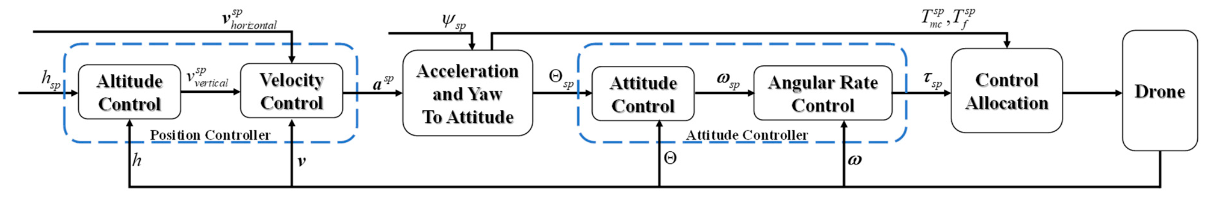
\includegraphics[width=1\textwidth]{Cap4/control.png}
    \caption{Arquitetura PID cascata \cite{Hu2024}.}
    \label{fig:cascata}
\end{figure}

A Figura~\ref{fig:cascata} apresenta a estrutura completa, da referência de comando até os atuadores. O fluxo, da malha mais externa para a mais interna, é:
\begin{itemize}
    \item \textbf{Controlador de posição} (controle de altitude + controle de velocidade): a partir da altitude de referência $h_{sp}$ e da velocidade horizontal de referência $\mathbf{v}^{sp}_{hor}$, realimentado pela altitude $h$ e pela velocidade $\mathbf{v}$ medidas, gera uma \emph{aceleração de referência} $\mathbf{a}^{sp}$;
    \item \textbf{Conversão de aceleração e guinada em atitude}: combina a aceleração de referência $\mathbf{a}^{sp}$ com a guinada de referência $\psi_{sp}$ para produzir a \emph{atitude de referência} $\Theta_{sp}$;
    \item \textbf{Controlador de atitude} (controle de atitude + controle de velocidade angular): a partir de $\Theta_{sp}$ gera a velocidade angular de referência $\boldsymbol{\omega}_{sp}$ e, desta, o \emph{momento de referência} $\boldsymbol{\tau}_{sp}$, realimentado pela atitude $\Theta$ e pela velocidade angular $\boldsymbol{\omega}$ medidas;
    \item \textbf{Alocação de controle}: converte o momento de referência $\boldsymbol{\tau}_{sp}$ e o empuxo total nos comandos individuais dos atuadores, fechando a cadeia até o drone, conforme a matriz de alocação deduzida no Capítulo~2.
\end{itemize}

A malha mais interna de velocidade angular corresponde justamente à dinâmica identificada nas seções anteriores, onde o modelo de taxa estimado por OEM é a planta sobre a qual essa malha é projetada, de modo que a qualidade da identificação reflete-se diretamente no desempenho do controle de atitude. Modelos de planta mais sofisticados, que capturam efeitos aerodinâmicos por abordagens híbridas combinando princípios físicos e aprendizado de máquina \cite{Bauersfeld2021}, são possíveis, porém o modelo de corpo rígido identificado mostra-se suficiente para o controle em torno do voo pairado. Cada malha é implementada por um controlador PID com saturação, projetado nas seções seguintes.

A arquitetura da Figura~\ref{fig:cascata} serve como referência conceitual geral. Neste trabalho adotou-se uma realização simplificada e desacoplada dela, suficiente para o controle em torno do voo pairado e coerente com o modelo identificado. As simplificações são:
\begin{itemize}
    \item cada eixo é tratado como uma malha SISO independente, o que se justifica pelo acoplamento cruzado desprezível do modelo linear, em que o momento de guinada gera sobre a rolagem apenas $\Gamma_4\approx0{,}27$ contra $\Gamma_3\approx21{,}3$ na própria diagonal (cerca de $1\%$), já que o produto de inércia $J_{xz}$ é ínfimo, fato que a simulação confirma adiante;
    \item a atitude é controlada por um PD em cada eixo, proporcional ao erro de ângulo e derivativo na velocidade angular medida, de modo que a malha de velocidade angular fica embutida no termo derivativo, sem uma referência $\boldsymbol{\omega}_{sp}$ explícita;
    \item da velocidade horizontal controla-se apenas a componente de avanço, com a rolagem regulada em zero, e o comando de atitude resulta diretamente do erro de velocidade, sem o estágio intermediário de aceleração de referência $\mathbf{a}^{sp}$;
    \item a altitude é regulada diretamente pelo empuxo total, com realimentação direta do peso.
\end{itemize}

\section{Projeto de Controladores PID}

Cada malha da cascata foi projetada de forma independente por alocação de polos sobre o modelo de taxa identificado por OEM, linearizado em torno do voo pairado conforme o Apêndice~\ref{ap:linearizacao}. Os coeficientes que entram no projeto são, portanto, lidos diretamente das matrizes $A$ e $B$ desse modelo linear, de modo que a qualidade da identificação propaga-se para os ganhos obtidos. O procedimento é direto. Para cada malha escolhe-se uma frequência natural $\omega_n$ e um fator de amortecimento $\zeta$, que traduzem a especificação de desempenho desejada, ou seja, a rapidez de resposta e o sobressinal aceitável. Em seguida igualam-se os coeficientes do polinômio característico de malha fechada aos do polinômio de segunda ordem de referência $s^2+2\zeta\omega_n s+\omega_n^2$, e os ganhos resultam dessa igualdade.

As malhas internas de atitude foram projetadas mais rápidas que as externas de velocidade e altitude, com separação de banda de cerca de quatro vezes. Assim a malha interna responde de modo praticamente instantâneo para a malha externa, e ambas podem ser ajustadas sem interação significativa.

\subsection{Malhas de atitude}

A dinâmica de atitude usada no projeto vem da linearização, em torno do voo pairado, das equações rotacionais identificadas nas seções anteriores. Tomando a rolagem como exemplo, a Equação~\eqref{eq:p_dot} fornece: 

$\dot p=\Gamma_1 pq-\Gamma_2 qr+\Gamma_3\tau_x+\Gamma_4\tau_z-c_p\,p$. 
Perto do hover as velocidades angulares são pequenas, de modo que os produtos giroscópicos ($pq$, $qr$) e o acoplamento de guinada ($\Gamma_4\tau_z$) tornam-se desprezíveis, restando $\dot p\approx -c_p\,p+\Gamma_3\,\tau_x$. Como, nessa condição, a cinemática de Euler reduz-se a $\dot\phi=p$, segue que $\ddot\phi\approx-c_p\,\dot\phi+\Gamma_3\,\tau_x$. Cada eixo de atitude assume, assim, a forma de segunda ordem
\begin{equation}
\ddot{\alpha}=-a\,\dot{\alpha}+b\,\tau,
\label{eq:att-2ord}
\end{equation}
em que $\alpha$ é o ângulo, $a$ o arrasto angular e $b$ a efetividade de controle. O arrasto $a$ é o coeficiente $c_p$, $c_q$ ou $c_r$ identificado, e a efetividade $b$ é o termo de inércia correspondente ($\Gamma_3$ na rolagem, $1/J_y$ na arfagem e $\Gamma_8$ na guinada), ambos lidos diretamente das matrizes do modelo linear na forma $a=-A_{ii}$ e $b=B_{ij}$.

A lei é um PD na forma $\tau=K_p(\alpha_c-\alpha)-K_d\,\dot{\alpha}$, cujo polinômio de malha fechada é $s^2+(a+bK_d)\,s+bK_p$. Igualando à forma de referência obtêm-se os ganhos
\begin{equation}
K_p=\frac{\omega_n^2}{b}, \qquad K_d=\frac{2\zeta\omega_n-a}{b}.
\label{eq:gain-att}
\end{equation}
A Tabela~\ref{tab:gain-att} apresenta, por eixo, os coeficientes $a$ e $b$ do modelo, a especificação $(\omega_n,\zeta)$ e os ganhos obtidos.

\begin{table}[ht]
\centering
\caption{Coeficientes do modelo, especificação e ganhos das malhas de atitude.}
\label{tab:gain-att}
\begin{tabular}{l c c c c c c}
\toprule
Eixo & $a$ [s$^{-1}$] & $b$ [(kg$\cdot$m$^2)^{-1}$] & $\omega_n$ [rad/s] & $\zeta$ & $K_p$ & $K_d$ \\
\midrule
Rolagem ($\phi$)   & 6,85 & 21,33 & 6,0 & 0,8 & 1,69 & 0,13 \\
Arfagem ($\theta$) & 4,68 & 10,71 & 6,0 & 0,8 & 3,36 & 0,46 \\
Guinada ($\psi$)   & 0,81 &  7,93 & 2,5 & 0,8 & 0,79 & 0,40 \\
\bottomrule
\end{tabular}
\end{table}

\subsection{Malha de velocidade de avanço}

Com a atitude interna rápida, a velocidade longitudinal segue $\dot{u}\approx-g\,\theta$. Comanda-se o ângulo de arfagem por um PI na forma $\theta_c=-\left(K_p\,e_u+K_i\!\int e_u\,dt\right)/g$, o que leva à dinâmica $s^2+K_p\,s+K_i$ e, portanto, aos ganhos
\begin{equation}
K_p=2\zeta\omega_n, \qquad K_i=\omega_n^2.
\label{eq:gain-u}
\end{equation}
Nesta malha a especificação fixa diretamente os ganhos, sem depender da planta, como mostra a Tabela~\ref{tab:gain-u}.

\begin{table}[ht]
\centering
\caption{Valores de projeto e ganhos da malha de velocidade de avanço.}
\label{tab:gain-u}
\begin{tabular}{l c}
\toprule
Grandeza & Valor \\
\midrule
$g$ [m/s$^2$]      & 9,81 \\
$\omega_n$ [rad/s] & 1,5  \\
$\zeta$            & 0,9  \\
$K_p$              & 2,70 \\
$K_i$              & 2,25 \\
\bottomrule
\end{tabular}
\end{table}

\subsection{Malha de altitude}

A altitude é um duplo integrador acionado pelo empuxo, $\ddot{h}=\delta T/m$, controlado por um PID com realimentação direta do peso $m g$. Os ganhos resultam em
\begin{equation}
K_p=m\,\omega_n^2, \qquad K_d=2\,m\,\zeta\,\omega_n.
\label{eq:gain-h}
\end{equation}
O termo integral é mantido nulo, uma vez que a realimentação direta de $mg$ já cancela o erro de regime. A Tabela~\ref{tab:gain-h} reúne os valores empregados.

\begin{table}[ht]
\centering
\caption{Valores de projeto e ganhos da malha de altitude.}
\label{tab:gain-h}
\begin{tabular}{l c}
\toprule
Grandeza & Valor \\
\midrule
$m$ [kg]           & 1,993 \\
$\omega_n$ [rad/s] & 2,0  \\
$\zeta$            & 0,9  \\
$K_p$              & 7,97 \\
$K_d$              & 7,18 \\
\bottomrule
\end{tabular}
\end{table}

Por fim, dois limites garantem a operação segura do controlador. O ângulo de arfagem comandado pela malha de velocidade é saturado em vinte graus, e os integradores de velocidade e de altitude são limitados, com anti-windup condicional que congela a integração enquanto o comando permanece saturado, conforme a Tabela~\ref{tab:ctrl-lim}.

\begin{table}[ht]
\centering
\caption{Limites de saturação e anti-windup do controlador.}
\label{tab:ctrl-lim}
\begin{tabular}{l c}
\toprule
Limite & Valor \\
\midrule
Ângulo de arfagem comandado ($\theta_c$) & $\pm 20^\circ$ \\
Integrador de velocidade & $\pm 5{,}0$ \\
Integrador de altitude   & $\pm 5{,}0$ \\
\bottomrule
\end{tabular}
\end{table}

\section{Simulação no Modelo Linear}

Para avaliar a arquitetura projetada, a malha fechada foi simulada sobre o mesmo modelo linearizado em torno do voo pairado empregado no projeto dos ganhos, cujos coeficientes vêm da identificação por OEM apresentada nas seções anteriores. O estado é integrado por Runge--Kutta de quarta ordem com passo de $10$\,ms, partindo do voo pairado nivelado, e o controlador em cascata recebe uma sequência de degraus desacoplados que exercita as três malhas externas: altitude de $0$ para $2$\,m em $t=1$\,s, velocidade longitudinal de $0$ para $3$\,m/s em $t=8$\,s e guinada de $0$ para $30^\circ$ em $t=16$\,s.

\subsection{Saturação dos atuadores}

Diferentemente de uma simulação puramente linear, em que a planta receberia o comando $[\,T,\ \tau_x,\ \tau_y,\ \tau_z\,]$ de forma irrestrita, aqui o limite físico dos motores é imposto dentro da malha. A cada passo o comando do controlador é alocado nos quatro empuxos individuais pela inversa da matriz de alocação~$B$ deduzida no Capítulo~2,
\begin{equation}
\mathbf{T}_{mot}=B^{-1}\,[\,T,\ \tau_x,\ \tau_y,\ \tau_z\,]^{\mathsf{T}} ,
\label{eq:aloc-inv}
\end{equation}
e cada empuxo é convertido no respectivo sinal de PWM pela inversão do modelo de motor da Equação~\eqref{eq:motor-thrust}. O PWM é então saturado na faixa física $[\,1200,\ 2000\,]\ \mu$s, em que o piso de $1200\ \mu$s corresponde à marcha lenta do rotor armado, abaixo da qual o motor não mantém rotação, e reconvertido em empuxo efetivo; aplicando novamente~$B$, recompõe-se o esforço $[\,T,\ \tau_x,\ \tau_y,\ \tau_z\,]_{ef}$ que a planta de fato recebe. Assim a resposta de malha fechada reflete o que os atuadores conseguem entregar, e não o comando ideal. Esse limite soma-se às proteções já internas ao controlador, a saturação do ângulo de arfagem comandado em $\pm 20^\circ$ e o anti-\textit{windup} condicional dos integradores, da Tabela~\ref{tab:ctrl-lim}.

\subsection{Resultados}

A Figura~\ref{fig:sim-control-linear} apresenta a resposta completa. As três malhas externas seguem suas referências com erro de regime praticamente nulo: a altitude estabiliza em $2$\,m com sobressinal de $0{,}1\%$, a velocidade de avanço em $3$\,m/s com $14{,}9\%$ e a guinada em $30^\circ$ com $1{,}5\%$. O sobressinal mais alto na velocidade decorre da saturação do ângulo de arfagem comandado, que atinge o limite de $\pm 20^\circ$ durante a aceleração (visível no painel de atitude, em que $\theta_c$ ultrapassa $\theta$). As malhas internas de atitude permanecem bem amortecidas, com rolagem máxima de apenas $1{,}27^\circ$, evidenciando o desacoplamento entre os eixos.

O painel inferior mostra o PWM dos quatro motores. O empuxo total exigido alcança $30{,}2$\,N no degrau de altitude, próximo do teto de $4\times 7{,}65 = 30{,}6$\,N do conjunto, o que leva os quatro motores ao limite superior de $2000\ \mu$s. Na manobra de guinada o binário diferencial necessário empurra um par de motores ao limite superior e o outro ao inferior ($1200\ \mu$s, a marcha lenta), o único instante em que se observa saturação inferior. No total, o comando demandado excursiona de $594$ a $2248\ \mu$s,fora da faixa física, mas a saturação atua em apenas $1{,}9\%$ dos instantes, concentrados nesses dois transitórios mais agressivos. Mesmo nesses trechos a malha permanece estável e o seguimento é preservado, com um pequeno afundamento de altitude durante a guinada decorrente do acoplamento entre o binário de guinada e o empuxo. O resultado confirma que os ganhos projetados produzem uma resposta rápida e bem amortecida e que a autoridade de controle dos motores é suficiente para as manobras consideradas, esgotando-se apenas nos picos de exigência simultânea.

\begin{figure}[ht]
    \centering
    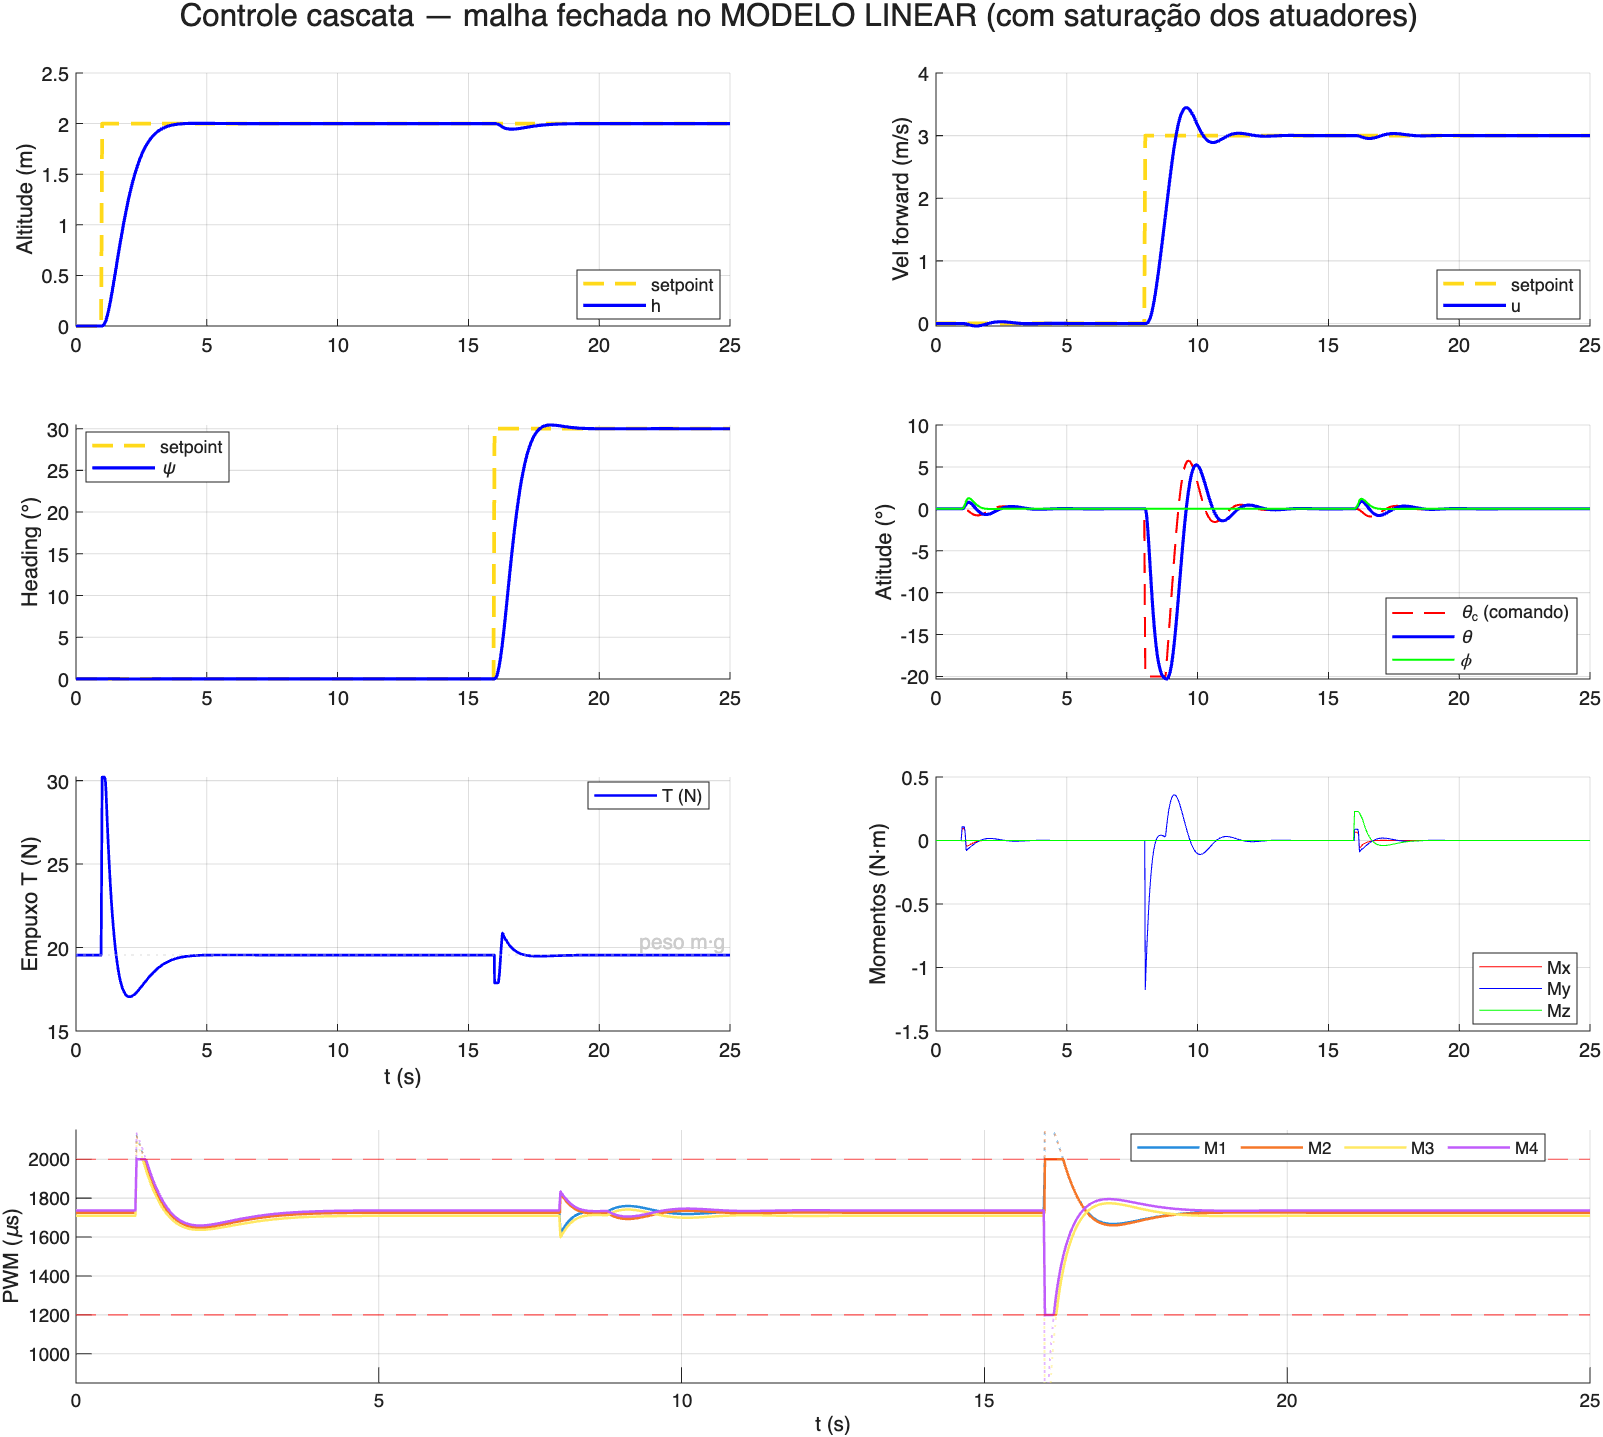
\includegraphics[width=1\textwidth]{Cap4/sim_control_linear.png}
    \caption{Resposta de malha fechada do controle em cascata sobre o modelo linear, com saturação dos atuadores.}
    \label{fig:sim-control-linear}
\end{figure}